\chapter{System-Level Design}

	\section{Overview}
	
	The mission architecture of the system is shown in \Cref{SLsketch}. This diagram shows the overall goal of the project.The vehicle traverses a field by following a path and avoiding any objects that may be in its way. This will be done with the sensors that are attached to the vehicle, as shown. Information about the status of the sensors, the speed and the vehicle�s performance will be relayed to the on-board microprocessors (Edison). This information will then be saved and inputted into an autopilot navigation system and obstacle avoidance control algorithm. Multiple Edison microprocessor boards will be necessary so that we do not have any issues with data processing and backlogging. The information saved on the processor will be able to be downloaded as a .txt file to be viewed by the user. This makes troubleshooting easier. A simple breakdown of this process is shown in \Cref{Block}. The vehicle will be able to make a decision to change course in a minimal amount of time. Our additions to the vehicle will be able to interface with the previous system. Our Edison processors will interact with the Arduino microcontrollers currently on the board to control the vehicle�s actuators. \Cref{oldBlock} is the previous years simplified block diagram, and this will help give a general understanding of the entire system.
	
\begin{figure}[h!]
\begin{center}
%\includegraphics[width=\textwidth]{Figures/.png}
\caption[System Level Sketch]{Shown is system level sketch, or mission architecture.}
\label{SLsketch}
\end{center}
\end{figure}

\begin{figure}[h!]
\begin{center}
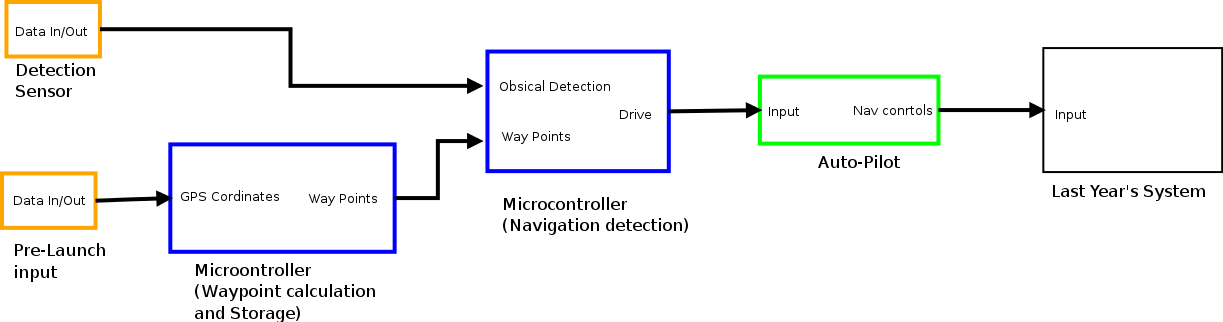
\includegraphics[width=\textwidth]{Figures/RSL_Rover_BlockDiagram.png}
\caption[Component Block Diagram]{Shown is a simplified component block diagram showing general signal flow. It abstracts away all of the previous years system into a single block on diagram because all work is to be done upstream of their work.}
\label{Block}
\end{center}
\end{figure}

\begin{figure}[h!]
\begin{center}
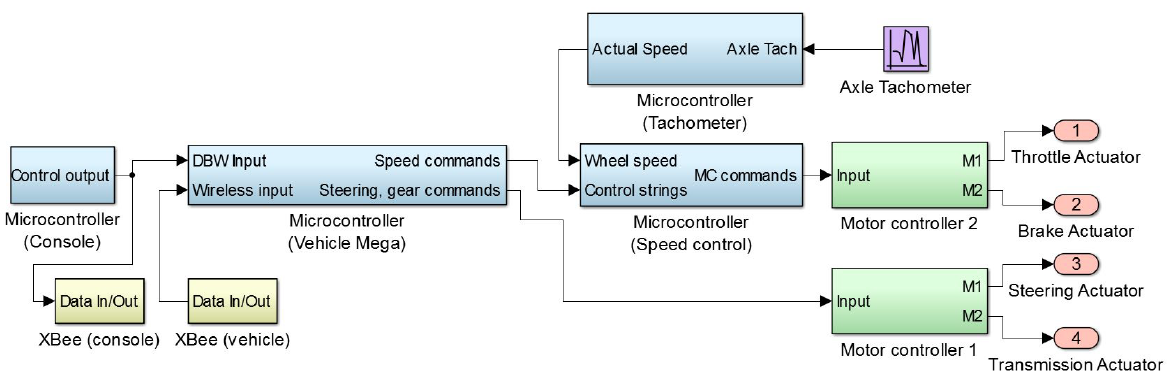
\includegraphics[width=\textwidth]{Figures/PreviousCBD.png}
\caption[Previous Year's Component Block Diagram]{Simplified block diagram of previous work.}
\label{oldBlock}
\end{center}
\end{figure}


	\section{Customer Definition and Needs}
	The objective of this project is to retrofit the current unmanned land vehicle with sensors and microprocessors to allow the vehicle to have autonomous capabilities. The process of doing so should be well documented and the final product should be easy to use. This is necessary so that future students may use the vehicle with a relatively small learning curve. The vehicle has some built in constraints that are not fixable. These include: the weight, size, engine power, etc. However, the vehicle is still relatively flexible. Our team will be able to customize the type of sensors we use and determine the user interface, the vehicle speed, accuracy, robustness, and cost to fit in line with the customer needs.

There are two customers in mind for our project. The first one is the Robotics Systems Laboratory. Future undergraduate, graduate and Ph.D. students will be able to use the vehicle to expand their knowledge of control systems, vehicle control, and etc. Our second customer is a group of farmers in rural locations in California. Their lack of resources makes it hard for them to compete versus large farming corporations. We hope that our vehicle will be able to assist them in the detection of underground pipes that may be hidden in their plots of land. The final product needs to be easy to use and understandable. Thus, the algorithms used to control the vehicle to be simple and robust enough that users with limited knowledge will not have any issues. A friendly user interface will allow the user to control aspects of the vehicle without actually having to change the code. Quality of the parts is also an issue. We want to retrofit the system with the best parts that our budget allows us; this will decrease the maintenance needed in the future and make it easier for the customer to trust the system. Also, by using parts manufactured by well-establish companies, the components being used will become less likely to be obsolete in the future.

Safety is a large concern for us. Because this system will be autonomous, extra precautions must be takenbecause a mistake could result in a serious injury or even death. Several safety systems will be implemented to protect both the user and the vehicle. These include ``dead man'' switches that shut off the system if the connection to a sensor is lost, warning signals/sounds from the vehicle, and a maximum speed limit of the vehicle in relation to he environmental conditions and sensor quality. The safety of the end user is our primary concern.
	\section{System Level Requirements}
	The system requirements from the previous year are still valid. The project will have four focuses:
	
\begin{compactitem}
	\item Navigation Control: Vehicle will take in GPS coordinates and use those to traverse a plot of land or path. When following a predetermined route, the vehicle will not deviate more than 0.5 meters. A closed loop feedback control system will be implemented to read the feedback and make adjustments if necessary.
	\item Velocity Control: The vehicle will try to maintain a 10 mph speed which equates to approximately to 3.6 acres per hour. The speed can be adjusted depending on the terrain, weather conditions and visibility. The maximum speed will not exceed 13 mph.
	\item Sensor Control: Limit the amount of false alarms from the RADAR system to 1\%. Sensors will be managed by a control algorithm. The information will be sent to the micro-processors, ideally only one or two sensors per microprocessor to prevent a backup of information. The latency between the sensor and microprocessor should be less than 500ms.
	\item Interface/Data Storage: To make troubleshooting easy, we wish to have the vehicle generate a .txt file every time the vehicle and status.
\end{compactitem}

	\section{Benchmarking Results}
	{\bf coming soon}

	\section{Functional Analysis}
	The project is broken into four major subsystem:
\begin{enumerate}
	\item Navigation
	\item Sensor Interfacing
	\item User Interface
	\item Safety
\end{enumerate}

All of these subsections are intertwined in some way, but it�s easier to understand the work that needs to be done on each one if it is broken down. This also helps us prioritize which one these we find the most important and how they affect the other subsystems.

The first subsystem, is the Navigation system. We will be using an off the shelf auto pilot system. This APM comes built in with GPS capabilities and a compass. The APM will be interfaced with the pre-existing Arduinos that control the actuators. The information that is being sent to the APM will be interpreted and used to perform the correct actions.

The second subsystem are how the sensors are going to interface with each other. We will have several array of sensors in order to limit the amount of false alarms and get the most precise information possible. The information will be sent to the Edison boards for processing and that information will be relayed to the APM system.

The third subsystem is the user interface. We want our project to be easy to use for people that do not have a large amount of technical data, so we need to remove any of the unnecessary information that may be presented. We will be using the open-source software that comes with the APM that allows you to set your path. We also will allow the users to pull data from the Edison boards after the vehicle has completed its task for system diagnostics.

The fourth subsystem is safety. This includes hardwires and software automatic shutoffs. Because the system is autonomous we need to have a way to stop the process from a safe distance if the vehicle malfunctions. We will also implement code that will shut off the system if any of our sensors are unable to send information to the Edison. How the wiring is done is also important to safety; it must be made sure that none of those connections will come loose in the driving process.

	\section{System Level Issues and Trade-offs}
	
		{\bf coming soon}

	\section{Team and Project Management}
	
		{\bf coming soon}

		%\subsection{Initial Team Goals}
		
		%\subsection{Reflection on Team Goals}
		
		%\subsection{Mitigating Project Challenges and Working within Constraints}
		
		%\subsection{Budget}
		
		%\subsection{Timeline}
		
		%\subsection{Design Process}
		
		%\subsection{Risks and Mitigations}
		
		%\subsection{Team Management}